%CONCEITOS---------------------------------------------------------------
\chapter{CONCEITOS}
\label{chap:conceitos}
O presente capítulo abordará os conceitos necessários para uma melhor compreensão dos artifícios utilizados para tratar o problema apresentado no Capítulo \ref{chap:introducao}, assim como uma
explanação sobre os extratores de características de imagens que serão utilizados e o estado da arte atual.

\section{ESPAÇOS MÉTRICOS} %TODO Ampliar
\label{sec:espmet}
Uma métrica em um conjunto $\mathbb{S}$ é uma função $d:\mathbb{S}$ $\times$ $\mathbb{S}$ $\rightarrow$ $\mathbb{R^{+}}$ que associa a cada par 
ordenado de elementos ($s_1$, $s_2$) um número real $d$($s_1$,$s_2$) chamado de distância de $s_1$ a $s_2$ \cite{Lima1977}.\par
Um espaço métrico $\mathbb{M}$ é um par <$\mathbb{S}$, $d$> onde $\mathbb{S}$ é um conjunto de elementos e $d$ é uma métrica
(ou função de distância). Esta distância $d$($s_1$,$s_2$) pode ser compreendido como uma medida de dissimilaridade entre dois elementos.
Quanto menor esta distância entre dois elementos, mais semelhantes eles são.
\begin{mydef}
 \label{def:espmet}
  Seja $\mathbb{S}$ um conjunto não-vazio de elementos e $d$($s_1$,$s_2$) uma métrica definida sobre $\mathbb{S}$ $\times$ $\mathbb{S}$.
   O par <$\mathbb{S}$, $d$> é chamado de espaço métrico desde que $d$ satisfaça as seguintes propriedades:\par
1. $d$($s_1$,$s_1$) = 0 (identidade);\par
2. Se $s_1$ $\neq$ $s_2$ ent\~ao $d$($s_1$,$s_2$) > 0 (n\~ao-negatividade);\par
3. $d$($s_1$,$s_2$) = $d$($s_2$,$s_1$) (simetria);\par
4. $d$($s_1$,$s_3$) $\leq$ $d$($s_1$,$s_2$) + $d$($s_2$,$s_3$) (desigualdade triangular)\\
onde $s_1$, $s_2$, $s_3$ $\in$ $\mathbb{S}$.
\end{mydef}
A importância prática do espaço métrico para este trabalho reside fortemente na quarta propriedade apresentada pela Definição \ref{def:espmet}. A desigualdade triangular é fundamentada na geometria euclidiana, 
onde a soma do comprimento de dois lados de um triângulo não pode ser superior ao comprimento do terceiro lado, como ilustra a figura \ref{fig:destri}.

\begin{figure}[H]
\centering
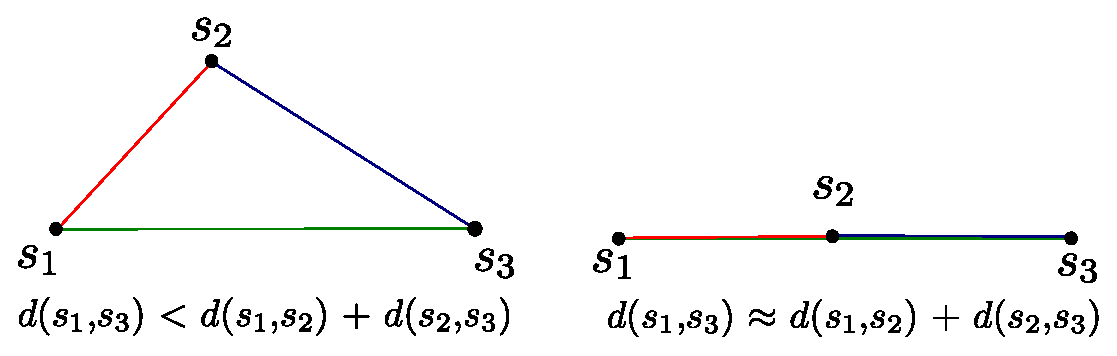
\includegraphics[width=.8\textwidth]{dados/figuras/desig_tri.eps}
\caption{Exemplo geométrico da desigualdade triangular}
\label{fig:destri}
\fonte{Autoria Própria}
\end{figure}

O emprego da desigualdade triangular neste trabalho será detalhado no capítulo \ref{chap:omni}.

\section{FUNÇÕES DE DISTÂNCIA}
\label{sec:funcdist}
Para verificar a similaridade entre dois elementos de um domínio, é utilizada uma função de distância. Esta função recebe como parâmetro um par
de elementos do conjunto e retorna o valor da dissimilaridade entre eles. Quanto mais próximo de zero, mais similares os elementos são.\par

A importância do uso de uma função de distância para este trabalho é fornecer uma métrica de comparação entre os elementos. Além de
necessária para a consulta por similaridade, a função de distância também é utilizada para evitar cálculos desnecessários, fornecendo uma métrica
empregada pela técnica Omni.\par

Dentre as funções de distância, será abordada a metrica Minkowski. Esta métrica é a mais utilizada para cálculos de índice de similaridade, e tem como resultado o valor da 
dissimilaridade entre dois elementos \cite{Jain1988}.
\begin{mydef}
\label{def:mink}
  Sejam $s_1 = \{s_{11},s_{12},...,s_{1n}\}$ e $s_2 = \{s_{21},s_{22},...,s_{2n}\}$ dois vetores de dimensionalidade $n$ pertencentes ao conjunto de
  elementos $\mathbb{S}$, a distância Minkowski entre esses dois elementos é dada por:
\begin{equation}
		d(s_1,s_2) = \sqrt[p]{\sum_{i=1}^{n}|s_{1i} - s_{2i}|^p}
\end{equation}
\end{mydef}
Para o caso em que $p = 2$ $(L_2)$, a distância Minkowski torna-se a tradicional distância euclidiana, amplamente utilizada para distância entre vetores.
%TODO Por que é utilizada a distância euclidiana? Por que a Minkowski é a mais utilizada para similaridade? É pertinente colocar L2?

\section{ESTRUTURAS DE INDEXAÇÃO}
\label{sec:index}
%TODO É necessário conceituar como é feito o acesso ao disco? Carregamento de dados? Bucket?
Dados complexos costumam apresentar tamanho físico muito elevado quando comparados com dados numéricos ou pequenas cadeias de caracteres, que são os tipos de dados
mais comuns em bancos de dados tradicionais. Para responder consultas que envolvam dados complexos, são necessários mais acessos a disco em relação a uma consulta
que envolva tipos de dados mais simples, como os previamente mencionados. Estes acessos são custosos e precisam ser reduzidos para um melhor desempenho do banco.\par %TODO Trocar custosos por outra palavra? 

Uma maneira de tornar o acesso a disco mais eficiente é evitar movimentar grandes porções do banco de dados do disco para a memória, fazendo o uso de índices dentro do banco de dados. 
Um índice em um SGBDR funciona de maneira semelhante a um índice de um livro. Para procurar um tópico específico, é possível consultar o índice no fim do livro e descobrir qual o número da página
correspondente ao tópico, contornando a necessidade da leitura sequencial do livro até o tópico procurado. Os índices são armazenados em ordem e apresentam um tamanho
muito menor do que um capítulo do livro, reduzindo o esforço necessário para a sua consulta \cite{Silberschatz2011}.\par
%TODO expandir

\section{EXTRATORES DE CARACTERÍSTICAS}
\label{sec:extcarac}
O principal foco deste trabalho é o emprego destas técnicas para bases de dados constituídas por imagens. Para isto, torna-se necessário o uso de uma miríade de extratores de características
das imagens, para um maior refinamento do uso de consultas por similaridade. Estas características podem se referir a: atributos visuais (cor, forma, textura), atributos lógicos (identificação
de elementos) e atributos semânticos (identificação de emoções humanas).\par

As características visuais podem ser utilizadas como histogramas de cores para a análise de cor, matrizes de co-ocorrência para a análise de textura e
métodos baseados em contorno para a análise de forma. Geralmente, consultas são feitas utilizando uma combinação destas características, e não apenas uma delas.\par

Dado uma palheta discreta de cores definida por alguns eixos de cor, o histograma de cores é obtido através da discretização das cores da imagem e contagem
do número de vezes que cada cor discreta ocorre na matriz da imagem \cite{Swain1991}. As vantagens do uso do histograma de cores é a sua simplicidade computacional e pouca
sensibilidade a alterações na imagem (rotação e translação), particularmente útil para a representação de objetos tridimensionais. Entretanto, duas imagens completamente 
diferentes podem apresentar o mesmo histograma de cores.\par

Para a análise de textura, o objetivo e conseguir distinguir regiões que apresentam cores similares (como folhagem e grama), analisando o padrão
de variação dessas cores. A técnica mais utilizada analisa conjunto de pares de pixels da imagem em tons de cinza e monta estruturas com informações características.
A principal estrutura utilizada nesta técnica é a "Matriz de co-ocorrência".\par %TODO Definir matriz de co-ocorrência. Principal importância da análise de textura?

Diversas medidas que podem ser extraídas destas matrizes de co-ocorrência estão presentes no trabalho de \cite{Haralick1973}. Os extratores de características das imagens utilizados 
neste trabalho são do framework Arboretum, desenvolvido pelo Grupo de Bases de Dados e Imagens (GBDI) da Universidade de São Paulo - campus São Carlos.





%TODO % Para entender e ajustar os métodos de consultas por similaridade para diferentes tamanhos e tipos de conjuntos de dados, além de comparar diversos métodos, é importante uma análise teórica dos diferentes
% métodos de acesso e técnicas de estimativa do custo computacional \cite{POLA2010}. O cálculo do custo das operações realizadas será feito utilizando operações com B-trees, as quais o banco fornece suporte
% ao modelo de custo.
